\chapter{Mathematical Model}
% REMOVE MATHEMATICAL??????
\section{Fixed Pitch Quadrotor}

In order to build and control a new type of quadrotor, a thorough understanding of the mathematics and physics involved is required. A mathematical model describing the physics and dynamics of both fixed pitch and variable pitch quadrotors is given.

\subsection{Frames of Reference}
In order to describe a quadrotor mathematically, a frame of reference is required. The quadrotor is observed from the ground, therefore it is most logical to use the ground as the frame of reference.\bigskip

A point of reference also has to be placed on the quadrotor, either at the center of gravity or the physical center of the quadrotor. For the control system, the most beneficial point of reference is the center of gravity. For a x-shaped frame it is natural to define the arms of the quadrotor as axes in the x and y directions. The third axis is the z-axis, which is orthogonal to x and y, representing up and down. \bigskip

\begin{figure}[H]
    \centering
    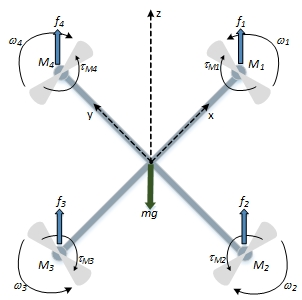
\includegraphics[width = 0.3\textwidth]{VAPIQ-PICTURES/MMFPQ.jpg}
    \caption{Quadrotor fixed pitch reference frame and forces}
    \label{fig:quadDynamics}
\end{figure}
\noindent
Fig. \ref{fig:quadDynamics} shows the quadrotor body frame of reference, "f" represents the lift force produced by the motor propeller combination. $\tau$ represents the torque and $\omega$ represents the rotational speed in rad/s.\bigskip

With these definitions in place, the rotational coordinate system can be defined. Fig. \ref{fig:quadAngles} shows the rotational angles around the body reference frame. The angle around the x axis is called roll $\phi$, the angle around the y axis is called pitch $\theta$ and last the angle around the z axis is called yaw $\psi$.\bigskip

\begin{figure}[H]
    \centering
    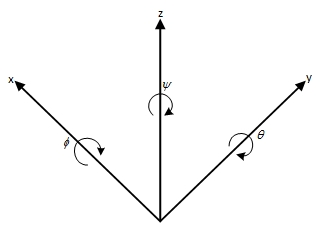
\includegraphics[width = 0.3\textwidth]{VAPIQ-PICTURES/RPJ.jpg}
    \caption{Rotational angles around the body frame}
    \label{fig:quadAngles}
\end{figure}
\bigskip
 
\subsection{Translational Motion}

To begin with, all the movement will be along the z-axis. If the origin is placed on the ground, the z-axis value will be the altitude of the quadrotor above zero. In this section, the mathematical model from the report from Charles Darwin University is used \cite{charlesdarwinuni}. \bigskip

In Fig. \ref{fig:quadDynamics} you can see the 4 forces and torques acting on the quadrotor and the gravitational force \textbf{(mg)} acting in the negative z-direction. If the quadrotor is at rest and the force is grater than the weight of the quadrotor, acceleration will occur. 
\begin{equation}
  f_{tot} = f_1 + f_2 + f_3 + f_4 - mg
\end{equation}
\\
From this equation the acceleration generated by the forces acting can be obtained 
\\
\begin{equation}
  f_{tot} = ma
\end{equation}
\\
In this equation, \textbf{m} is the mass of the quadrotor \textbf{kg} and \textbf{a} is the acceleration \textbf{$m/s^2$} .\bigskip

When the motors of the quadrotor gives the same amount of force, the quadrotor will move along the z-axis. For movement along the other axes, the force on one or more of the motors must be changed. The equations of motion are
\\
\begin{equation}
f_x = f_{tot}sin\theta
\end{equation}
\begin{equation}
f_y = f_{tot}sin\phi
\end{equation}
\begin{equation}
f_z = f_{tot}cos\theta cos\phi
\end{equation}
\\
From this the acceleration can be found by substituting
\\
\begin{equation}
a_x = \frac{f_{tot}sin\theta}{m}
\end{equation}
\begin{equation}
a_y = \frac{f_{tot}sin\phi}{m}
\end{equation}
\begin{equation}
a_z = \frac{f_{tot}sin\theta cos\phi}{m}
\end{equation}
\\
By integrating the acceleration, the velocity is obtained
\begin{equation}
v_x = \int a_xdt
\end{equation}
\begin{equation}
v_y = \int a_ydt
\end{equation}
\begin{equation}
v_z = \int a_zdt
\end{equation}
\\
And by integrating the velocity, the displacement
\begin{equation}
s_x = \int v_xdt
\end{equation}
\begin{equation}
s_y = \int v_ydt
\end{equation}
\begin{equation}
s_z = \int v_zdt
\end{equation}
\clearpage

\subsection{Rotational Motion}
Rotational motion in space is described by rotation around three axes. For rotational motion to occur, there must be an imbalance of forces applied to the quadrotor. Rotational motion can occur in many different ways, as shown in Table \ref{tabular:rotmot}. The table shows the different force imbalances and the resulting quadrotor motion. In this section, the mathematical model from \cite{charlesdarwinuni} is used. \bigskip

\begin{table}[h]
\centering
\caption{Rotational Motion}

\begin{tabular}{ |c|c|c|c| } 
 \hline \rowcolor{white}
 \textbf{Imbalance of forces} & \textbf{Roll} & \textbf{Pitch} & \textbf{Yaw} \\
 \hline
 None & - & - & - \\ 
 Opposite motors both increased & - & - & Pos/Neg \\ 
 Odd motors varied by opposite but equal amount & Pos/Neg & - & - \\ 
 Even motors varied by opposite but equal amount & - & Pos/Neg & - \\ 
 Adjacent motors both increased the same amount & Pos/Neg & Pos/Neg & - \\ 
 All motors at unequal amount & Pos/Neg & Pos/Neg & Pos/Neg \\ 
 \hline
\end{tabular}
    \label{tabular:rotmot}
\end{table} \\

From Table \ref{tabular:rotmot} you can see that yaw motion only occurs when there is an imbalance between diagonal motor pairs. The reason for this is that the yaw motion occurs when the net torque of the motor pairs are nonzero. If these torques do not cancel out, there is a resultant torque that causes rotation about the z-axis. 
\begin{equation}
    \label{eq:ttot}
    \tau_{tot} = \tau_1 + \tau_2 + \tau_3 + \tau_4
\end{equation}
\\
$\tau_{tot}$ is the resultant torque and $\tau_i$ is the torque caused by propeller $i$. Torque is measured in \textbf{Nm}. As the propeller rotates through the air, it causes drag that produces torque that is opposite to the propeller rotation. 
\begin{equation}
    \label{eq:kw2}
    f_i = k\omega_i^2
\end{equation}

\begin{equation}
    \tau_i = b\omega_i^2 + I_M\dot{\omega}_i
\end{equation}
\\
Where $f$ is the thrust, $k$ is the lift constant, $\tau_i$ is the torque produced by the drag force, b is the drag constant, $\omega$ is the angular velocity of the propeller, $\dot{\omega}$ is the angular acceleration and $I_M$ is the moment of inertia.\bigskip 

From these two equations it is clear that when the propellers are rotating at a constant velocity, the thrust and torque are proportional to the square of the angular velocity of the propellers. The moment of inertia contribution will be zero when the propeller is at a constant angular velocity.\bigskip 

When the conditions for yaw are met
\begin{equation}
    \label{eq:tyaw}
    \tau_{yaw} = \tau_{tot}\cdot l
\end{equation}
\\
Where $\tau_{yaw}$ is the torque in the yaw plane \textbf{(Nm) }and $l$ is the distance from the center of the motor to the center of the body \textbf{(m)}. This torque will produce an angular acceleration in the yaw plane. 
\begin{equation}
    \label{eq:ayaw}
    \tau_{yaw} = a_{yaw}\cdot I_{zz}
\end{equation}
\\
Where $a_{yaw}$ is the angular acceleration in $rad/s^2$ in the yaw plane and $I_{zz}$ is the moment of inertia in the yaw or $zz$ plane in $kg.m^2$. Substituting Equation. (\ref{eq:ayaw}) with (\ref{eq:ttot}) and (\ref{eq:tyaw}) we get the angular acceleration
\begin{equation}
    a_{yaw} = \frac{(\tau_1 + \tau_2 + \tau_3 + \tau_4) \cdot l}{I_{zz}}
\end{equation}
\\ 
Since all of these variables are known or can be calculated, the acceleration in the yaw plane can be determined. \bigskip

The torque can also be manipulated to produce roll motion in the xz-plane. For roll motion there has to be an unbalance between the left and right hand side, or other combinations, as seen in Table \ref{tabular:rotmot}. 
\begin{equation}
f_{roll} = f_2 - f_4
\end{equation}
\\
Where $F_{roll}$ is the resultant force in \textbf{Nm} in the roll direction. This will cause the quadrotor to have roll motion. 
\begin{equation}
\tau_{roll} = f_{roll}\cdot l
\end{equation}
\\
Where $\tau_{roll}$ is the resultant torque in \textbf{N} in the roll direction. Substituting the same way as for yaw, gives
\begin{equation}
    \label{eq:aroll}
    a_{roll} = \frac{\tau_{roll}}{I_{yy}}
\end{equation}
\\
Where $a_{roll}$ is the angular acceleration in $rad/s^2$ in the roll plane, and $I_{yy}$ is the moment of inertia in the roll or $yy$ plane in $kg.m^2$. \bigskip

Substituting equation (\ref{eq:kw2}) into equation (\ref{eq:aroll}) gives the expression for angular acceleration proportional to the motor speed
\begin{equation}
    \label{eq:aroll2}
    a_{roll} = \frac{(k\omega_2^2-k\omega_4^2)\cdot l}{I_{yy}}
\end{equation}\bigskip

Since the same logic applies to pitch movement the expression for acceleration in the pitch plane can be obtained from equation (\ref{eq:aroll2}). 
\begin{equation}
    a_{pitch} = \frac{(k\omega_1^2-k\omega_3^2)\cdot l}{I_{xx}}
\end{equation}
\\
Where $a_{pitch}$ is the angular acceleration in $rad/s^2$ in the pitch plane and $I_{xx}$ is the moment of inertia in the pitch or $xx$ plane in $kg.m^2$. \bigskip

Since the quadrotor is operating in discrete time, expressions for angular velocity and angular displacement in the roll, pitch and yaw directions can be found 
\begin{equation}
    \omega_{roll} = (a_{roll} - a_{roll-1})ts
\end{equation}

\begin{equation}
    \omega_{pitch} = (a_{pitch} - a_{pitch-1})ts
\end{equation}

\begin{equation}
    \omega_{yaw} = (a_{yaw} - a_{yaw-1})ts
\end{equation}
\\
\begin{equation}
    \theta = (\omega_{roll} - \omega_{roll-1})ts
\end{equation}

\begin{equation}
    \phi = (\omega_{pitch} - \omega_{pitch-1})ts
\end{equation}

\begin{equation}
    \psi = (\omega_{yaw} - \omega_{yaw-1})ts
\end{equation}
\\
Where $\omega_{roll}$, $\omega_{pitch}$ and $\omega_{yaw}$ are the angular velocities in $rad/s$ in the roll, pitch and yaw directions, and $\theta$, $\phi$ and $\psi$ are the angular displacement in $rad$ in the roll, pitch and yaw directions.  


\newpage
\section{Variable Pitch Quadcopter}

A variable pitch quadcopter has six degrees of freedom. $\phi$, $\theta$ and $\psi$ represents roll, pitch and yaw angles. $v_x$,$v_y$ and $v_z$ represents the flight velocities in the body frame. The force $f$ generated by the propellers and motors is given by

\begin{equation}
    f_{i} = k\alpha_i\omega_i^2
\end{equation}

Where $k$ is the aerodynamic constant,  $\alpha$ is the propeller pitch angle. and $\omega$ is the rotational speed of the propeller. Comparing this equation to equation (16), it can be seen that the only difference is the pitch blade angle $\alpha$.

\begin{figure}[H]
    \centering
    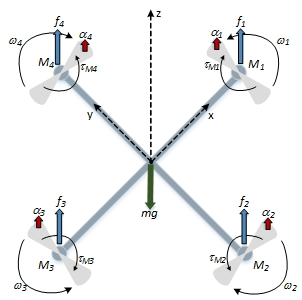
\includegraphics[width = 0.3\textwidth]{VAPIQ-PICTURES/MMVPQ.jpg}
    \caption{Variable Pitch Quadrotor, Frame Of Reference And Forces}
    \label{fig:ControllInputs}
\end{figure}

Figure \ref{fig:ControllInputs} shows the axes along with the lift force and torque vectors, pitch angle $\alpha$ and the rotational speed $\omega$. The total lift force in the z-axis generated by the motors and propellers is given by

\begin{equation}
   f_{z} = \sum_{i=1}^{4} f_{i} = \sum_{i=1}^{4} k\alpha_i\omega_i^2
\end{equation}

The drag produced by the motor and propeller can be approximated by the equation

\begin{equation}
   Q_j = b_{D1}\alpha_j^2\omega_j^2 + b_D_2\omega_j^2 + b_{D3}\alpha_j\omega_j
\end{equation}

Where $b_{D1}$,$b_{D1}$ and $b_{D1}$ is aerodynamical constants. The torques used to control roll, pitch and yaw moments can be described by the following equations.

\begin{equation}
   \tau_\phi = l(L_2-L_4) =lk(\alpha_2\omega_2^2-\alpha_4\omega_4^2)
\end{equation}

\begin{equation}
   \tau_\theta = l(L_3-L_1) = lk(\alpha_3\omega_3^2-\alpha_1\omega_1^2)
\end{equation}

\begin{equation}
   \tau_\psi = Q_1 + Q_3 - Q_4 - Q_2
\end{equation}

Where l is the distance from the propellers center to center of gravity of the quadcopter.\bigskip 

Comparing the variable pitch quadrotor equations for roll, pitch and yaw with the fixed pitch equations for roll, pitch and yaw, it can be seen that the only difference is the propeller pitch angle $\alpha$. This shows that the controller logic is quite similar for the variable pitch quadrotor as for the fixed pitch quadrotor.
\newpage
%%%%%%%%%%%%%%%%%%%%%%%%%%%%%%%%%%%%%%%%%%%%%%%%%
%%%%%%%%%%%%%%%%%%%%%%%%%%%%%%%%%%%%%%%%%%%%%%%%%

\section{Motor-Propeller Model}
The following motor model is derived based on the motor model described in the report from MIT \cite{MITvpp}. The motor model presented is a simplified representation of a three phase motor described as a basic DC motor.\bigskip %En antagelse/forenkling gjør at vi bruker denne.

In order to make the motor model, different motor constants for the specific motors used in this project needs to be determined. These constants can be found in the datasheet \cite{AXI}, and are given in Tab. \ref{tab:motconst}.

\begin{table}[H]
\centering
\caption{Motor Constants}
\label{tab:motconst}
\begin{tabular}{ |c|c| } 
 \hline
 $K_v$ [rad/s/v] & 148.702 \\ 
 \hline
 R [$\Omega$] & 0.155 \\ 
 \hline
 $i_0$ [A] & 0.6 \\ 
 \hline
\end{tabular}
\end{table}
\noindent
A basic DC motor is modeled as a circuit with a voltage source in series with a resistor and an inductor. By applying Kirchhoff's laws, equation (\ref{eq:vRi}) is obtained. 

\begin{equation}
    \label{eq:vRi}
    v = Ri + L\frac{\partial i}{\partial t} + e
\end{equation} 

Where $R$ is the internal motor resistance, $i$ is the current, $L$ is the motor inductance and $e$ is the back EMF. The back EMF, $e$, can be described as

\begin{equation}
    e = \frac{\omega}{K_v}
\end{equation}

where $\omega$ is the rotational speed [rad/s] and $K_v$ is the voltage constant of the motor [rad/s/v]. The motor model can then be rewritten as

\begin{equation}
\label{eq:vRi2}
    v = Ri + L\frac{\partial i}{\partial t} + \frac{\omega}{K_v}
\end{equation}
\bigskip

The motor torque $\tau_M$ can be modeled as proportional to the difference between the current, $i$, and the no-load current, $i_0$, divided by the torque constant, $K_Q$.  
\begin{equation}
    \label{eq:tm}
    \tau_M = \frac{i - i_0}{K_Q}
\end{equation}
\bigskip

The motor dynamics can be modeled as a first order differential equation
\begin{equation}
    \label{eq:motordiff}
    I\dot{\omega} = \tau_M - \tau_L
\end{equation}
where $\tau_M$ represents the motor torque produced by the voltage source, the load torque, $\tau_L$, is produced by the propeller drag and $I$ is the moment of inertia of the rotating parts. \bigskip

When using small brushless motors, the inductance is typically very small compared to the physical response of the system and can be neglected \cite{MITvpp}. When neglecting the inductance, substituting equation (\ref{eq:vRi2}) and (\ref{eq:tm}) into equation (\ref{eq:motordiff}) yields the following equation for $\dot\omega$.

\begin{equation}
    \label{eq:iomega}
    I\dot{\omega} =\left[\left(u-\frac{\omega}{K_v}\right)\frac{1}{R}-i_0\right]\frac{1}{K_Q} - \tau_L
\end{equation}
\newpage

\subsection{Non Linear Motor-Propeller Model}

\begin{equation}
    \label{eq:nonlinear}
    L = \rho cR_p^3\omega^2C_{L\alpha}\frac{\alpha}{3}
\end{equation}

\begin{equation}
    \label{eq:tauL}
    \tau_L =  \rho cR_p^4\omega^2\left(\frac{C_{D0} + C_{Di}\alpha^2}{4} - \frac{C_{L\alpha}\alpha\omega}{3R_p}\right)
\end{equation}\bigskip

These two equations shows the lift $L$ and drag $T_L$ produced by the motor-propeller combination. From these two equations it is shown that the lift and the drag is affected by the motor speed $\omega$ and the propeller pitch angle $\alpha$. The remaining terms of the equations are constants. This shows that to change the lift, you have to change either the pitch angle $\alpha$ or the motor speed $\omega$. By changing and combining the remaining constants of equations (\ref{eq:nonlinear}) and (\ref{eq:tauL}), equations (\ref{eq:Lbl}) and (\ref{eq:lbd}) can be obtained. 

\begin{equation}
    \label{eq:Lbl}
    L = b_L\omega^2\alpha
\end{equation}

\begin{equation}
    \label{eq:lbd}
    \tau_L = b_{D_1}\omega^2 + b_{D_2}\omega^2\alpha^2 + b_{D_3}\omega\alpha
\end{equation}\bigskip

Where $b_L$, $b_{D1}$, $b_{D1}$ and $b_{D1}$ are estimated lift and drag coefficients. These coefficients are obtained from the Variable Pitch Quadcopter report from MIT \cite{MITvpp} using the same propellers. The coefficients were selected by first identifying a similar symmetrical, tapered propeller in the NACA(National Advisory Committee for Aeronautics) database of airfoils. The particular airfoil chosen was the NACA 009. Using software the coefficients Tab. \ref{tab:EsLiDrCo} were estimated by MIT.

\begin{table}[H]
\caption{Estimated Lift and Drag coefficients}
\label{tab:EsLiDrCo}
\centering
    \begin{tabular}{ c c c c} 
    \hline
            b_L & b_{D1} & b_{D2} & b_{D3}\\
            3.88e-07  & 9.96e-09 & 2.46e-10 & 4.33e-07 \\
    \hline
    \end{tabular}
\end{table}

Substituting equation (\ref{eq:lbd}) into equation (\ref{eq:iomega}) yields the following equation.

\begin{equation}
    \label{eq:linearized}
    I\dot{\omega} = \left[ \left(v - \frac{\omega}{K_v}\right) \frac{1}{R} - i_0 \right]\frac{1}{K_Q} - b_{D_1}\omega^2 - b_{D_2}\omega^2\alpha^2-b_{D3}\omega\alpha
\end{equation}
\\\\
This equation is the nonlinear differential equation for $\dot\omega$.

%%%%%%%%%%%%%%%%%%%%%%%%%%%%%%%%%%%%%%%%%%%%%%%%%
%%%%%%%%%%%%%%%%%%%%%%%%%%%%%%%%%%%%%%%%%%%%%%%%%

\newpage

\subsection{Linearized Motor-Propeller Model}

To develop further insights into the dynamics of the motor, such as response time and steady state values, equation (\ref{eq:linearized}) needs to be linearized. The nonlinear equation (\ref{eq:linearized}) can be linearized at near hover conditions, using $\omega_0$ and $\alpha_0$. $\omega_0$ and $\alpha_0$ is the start rotational speed and pitch angle at hover, there are a infinite number of possible combinations of these that will yield hover. The linearization used is taken from the report from MIT \cite{MITvpp}. This yields equation (\ref{eq:deltaomega}) and (\ref{eq:deltaL}) which is the resulting state-space system. 

\begin{equation}
\label{eq:deltaomega}
    \Delta\dot{\omega} = \left[-\frac{1}{RK_VK_QI}-\frac{2b_D_1\omega_0}{I}-\frac{2b_D_2\omega_0\alpha_0^2}{I}-\frac{b_3\alpha_0}{I}\right]\Delta\omega + \left[\frac{1}{RK_QI}\quad - \frac{2b_D_2\omega_0^2\alpha_0}{I} + \frac{b_d3\omega_0}{I}  \right] \begin{bmatrix}
       \Delta v            \\[0.2em]
       \Delta\alpha \\[0.2em]
     \end{bmatrix}
\end{equation}

\begin{equation}
\label{eq:deltaL}
    \Delta L = \left[2b_L\omega_0\alpha_0 \right]\Delta\omega + \left[0\quad b_L\omega_0^2\right]
    \begin{bmatrix}
        \Delta v \\
        \Delta\alpha
    \end{bmatrix}
\end{equation}

Solving the multiplications of the matrices, equations (51) and (52) are obtained. 

\begin{equation}
    \Delta\dot{\omega} = \left(-\frac{1}{RK_VK_QI}-\frac{2b_D_1\omega_0}{I}-\frac{2b_D_2\omega_0\alpha_0^2}{I}-\frac{b_{D3}\alpha_0}{I}\right)\Delta\omega + \frac{1}{RK_QI}\Delta v - \left(\frac{2b_D_2\omega_0^2\alpha_0}{I} - \frac{b_{D3}\omega_0}{I}\right)\Delta\alpha
\end{equation}

\begin{equation}
    \Delta L = 2b_L\omega_0\alpha_0\Delta\omega + b_L\omega_0^2\Delta\alpha
\end{equation}

This system has two inputs and one output, which makes it a MISO system (Multiple Input, Single Output). The two inputs are the change in applied motor voltage, $\Delta v$, and change in propeller pitch/angle, $\Delta\alpha$. The output of the system is the change in lift, $\Delta L$, produced by the propellers. Based on equation (\ref{eq:deltaomega}) and (\ref{eq:deltaL}), a state-space canonical form block diagram can be created. Fig. \ref{fig:canonical} shows this block diagram. 

\begin{figure}[H]
    \centering
    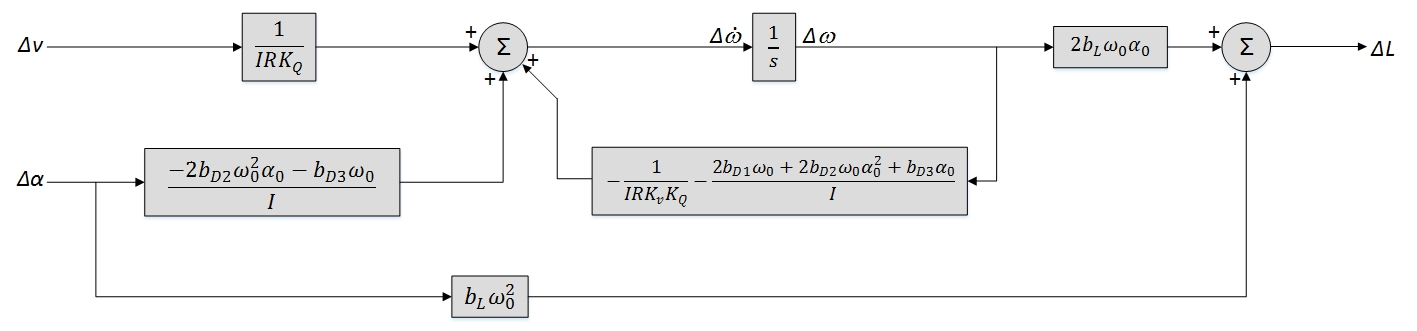
\includegraphics[width = 1\textwidth]{VAPIQ-PICTURES/canonicalblock.jpg}
    \caption{State-Space Canonical Block Diagram}
    \label{fig:canonical}
\end{figure}

\begin{equation}
\label{eq:AxBu}
    \dot x = Ax + Bu
\end{equation}

\begin{equation}
\label{eq:CxDu}
    y = Cx + Du
\end{equation}

Equation (\ref{eq:AxBu}) and (\ref{eq:CxDu}) shows a traditional representation of a state-space system. As seen from equation (\ref{eq:deltaomega}) and (\ref{eq:deltaL}), this is the state-space representation of the motor-propeller model, where $\Delta\dot\omega = \dot x$, $\Delta\omega = x$, $\Delta L = y$ and     \begin{bmatrix}
        \Delta v \\
        \Delta\alpha
    \end{bmatrix} $=u$. 

\begin{equation}
    A = \left[-\frac{1}{RK_VK_QI}-\frac{2b_D_1\omega_0}{I}-\frac{2b_D_2\omega_0\alpha_0^2}{I}-\frac{b_{D3}\alpha_0}{I}\right]
\end{equation}

\begin{equation}
    B = \left[\frac{1}{RK_QI}\quad - \frac{2b_D_2\omega_0^2\alpha_0}{I} - \frac{b_{D3}\omega_0}{I}  \right]
\end{equation}

\begin{equation}
    C = \left[2b_L\omega_0\alpha_0 \right]
\end{equation}

\begin{equation}
    D = \left[0\quad b_L\omega_0^2\right]
\end{equation}

Equation (\ref{eq:deltaomega}) and (\ref{eq:deltaL}) also yields A, B, C and D matrices for the state-space model. 

\newpage
\section{Simulation of State-Space Model}
\label{sec:simulation}
Based on the canonical form state-space block diagram from Fig. \ref{fig:canonical}, a Simulink simulation has been developed. This simulation will give an insight into the differences between fixed pitch and variable pitch quadcopters in terms of response time and the rotational speed of the motors. Fig. \ref{fig:simulink} shows the Simulink block diagram used. \bigskip

\begin{figure}[H]
    \centering
    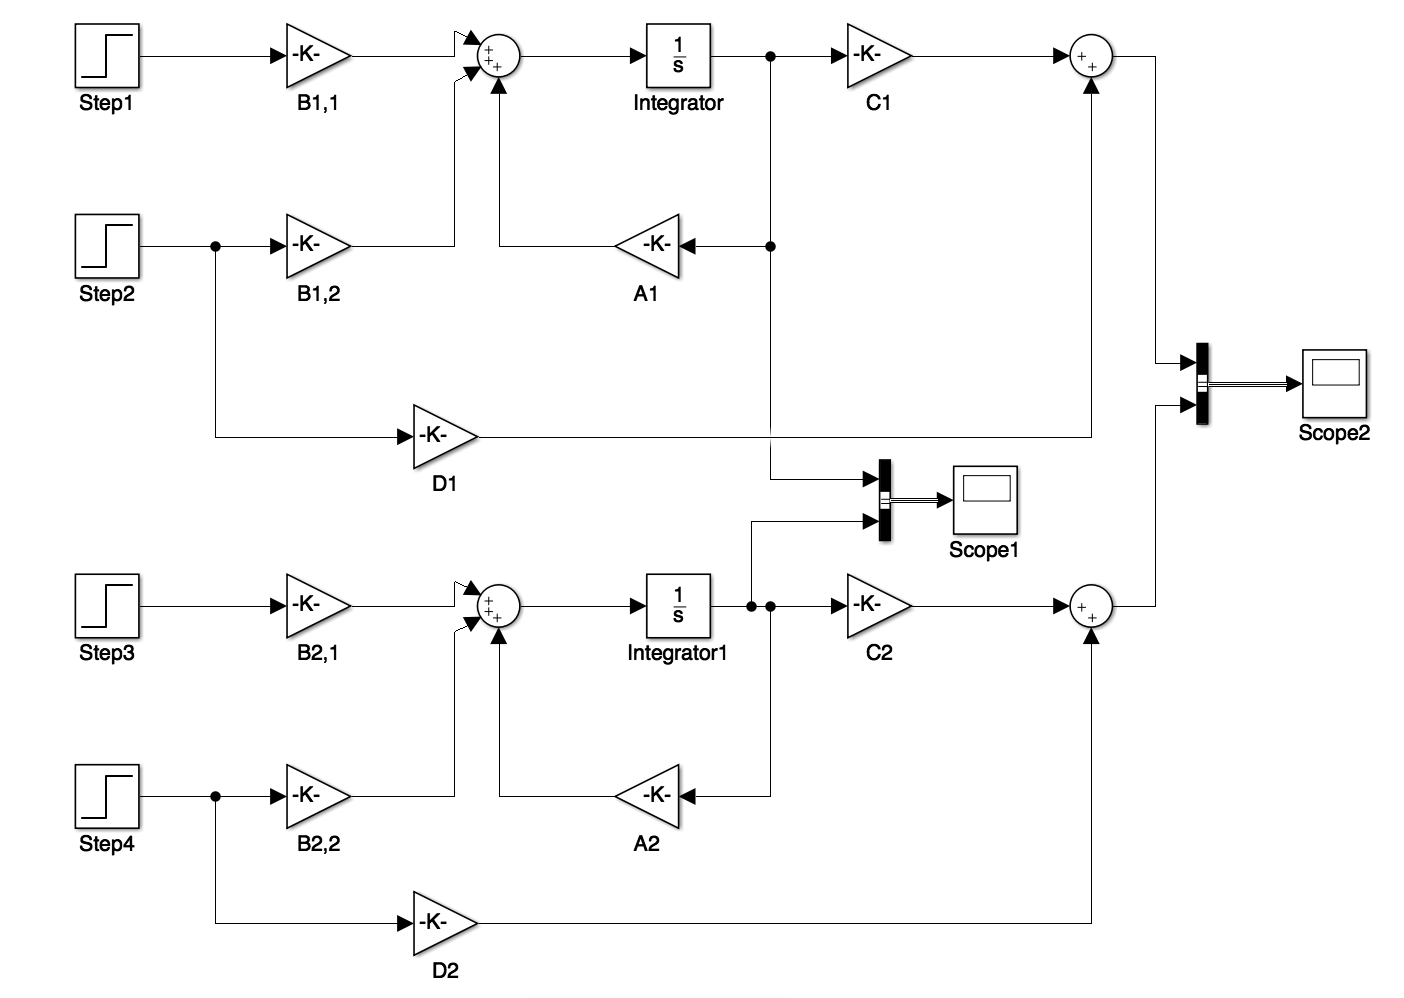
\includegraphics[width = 0.8\textwidth]{VAPIQ-PICTURES/simulinkblock.png}
    \caption{Simulink Block Diagram}
    \label{fig:simulink}
\end{figure}\bigskip

The simulation consists of two parts. The first part shows what happens when there is a change in pitch angle, and the other part shows what happens when there is a change in motor voltage. Step2 and Step3 are set to zero, so that the upper part of the block diagram will be the simulation of a change in voltage, and the bottom part of the block diagram will be the simulation of a change in pitch angle. \bigskip

There is placed one scope at the output and one scope after the integrator. The scope at the output shows the thrust response for both change in pitch and change in motor voltage. The scope after the integrator shows the rotational speed of the motors for both change in pitch and change in voltage. By adding a step response to the references, there will be a resulting thrust output and a rotational speed for the motors. \bigskip

\begin{figure}[H]
    \centering
    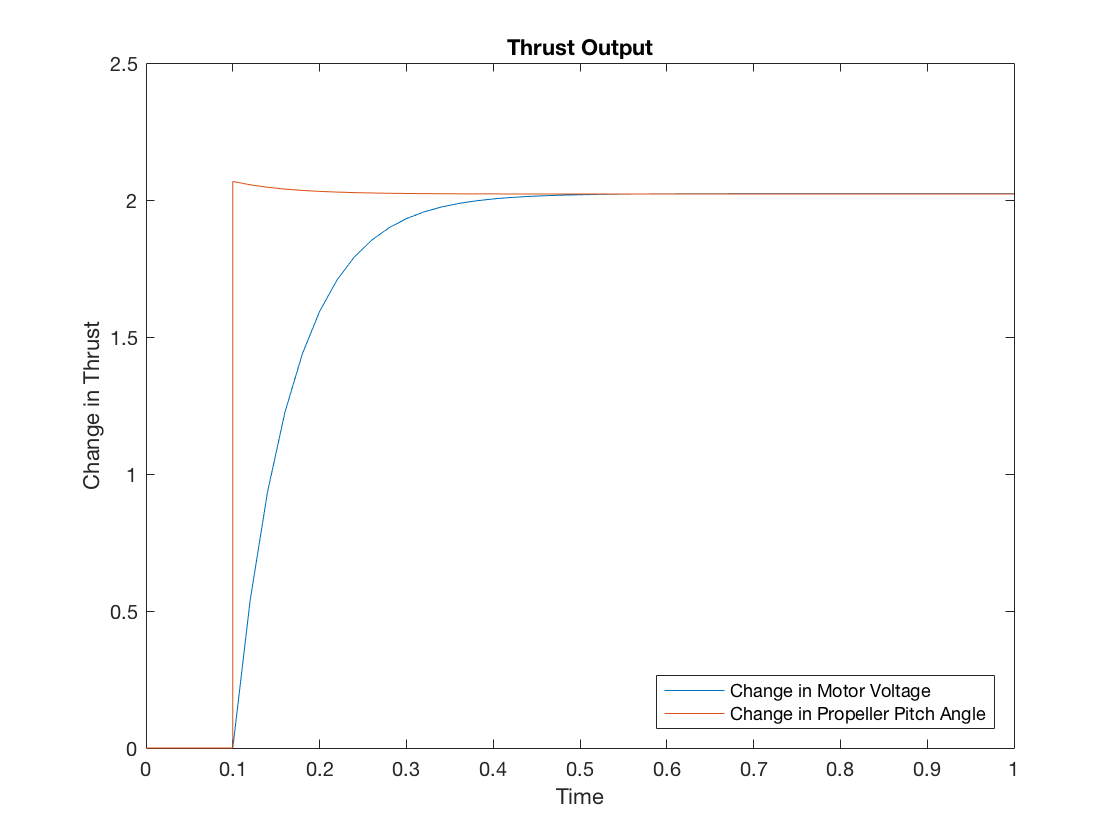
\includegraphics[width = 0.8\textwidth]{VAPIQ-PICTURES/thrustoutput.png}
    \caption{Thrust Output}
    \label{fig:thrust}
\end{figure}\bigskip

Fig. \ref{fig:thrust} shows the thrust output for a step response in both change in pitch angle and change in voltage. This graph is from the scope at the output (Scope2). The red graph shows the thrust output for a change in pitch angle. When the step response occurs, the thrust instantly increases. The servo actuation is modeled as instantaneous. From the red graph it is observed that there is a decrease in thrust after change in pitch. The decrease in lift is a result of the increased torque on the motors, which results in a decrease in rotational speed. The thrust stabilizes at the new steady state value. \bigskip

The blue graph in Fig. \ref{fig:thrust} shows the thrust output for a change in motor voltage. For a change in voltage, the thrust increases much slower than for a change in pitch. The reason for this is that it takes longer time to increase the rotational speed of the motors than to change the pitch angle of the propeller. \bigskip

\begin{figure}[H]
    \centering
    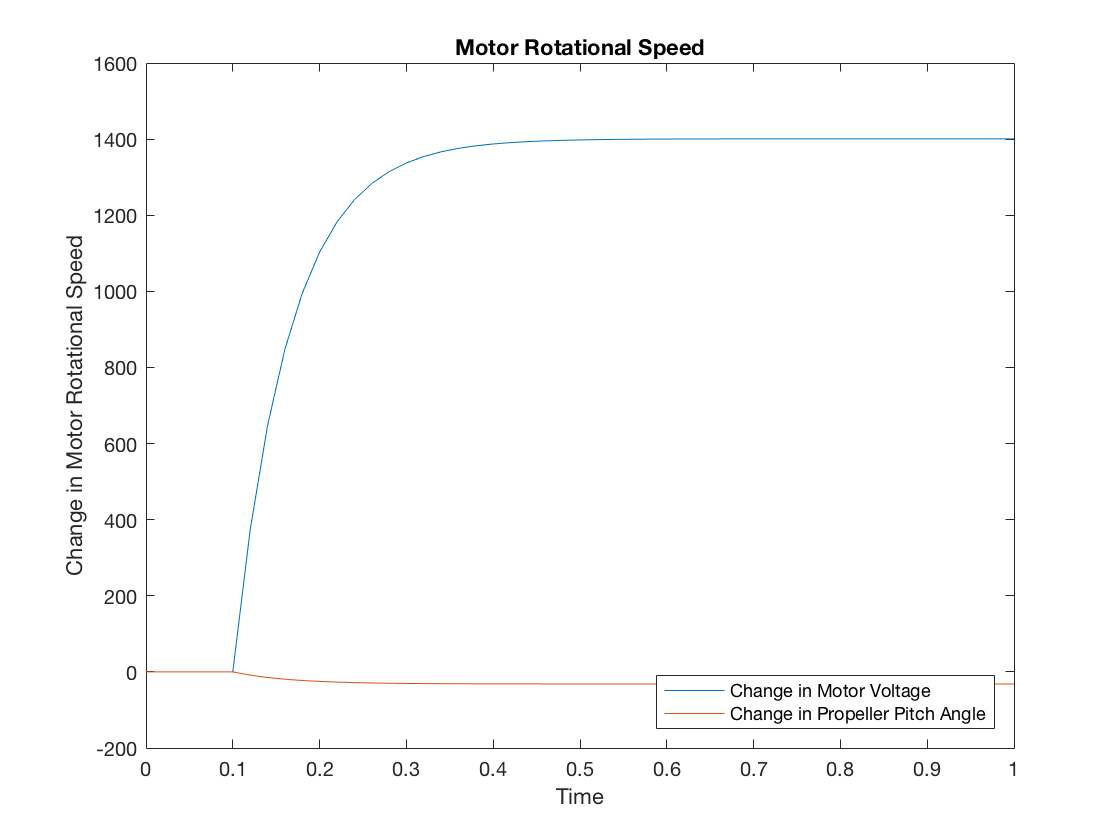
\includegraphics[width = 0.8\textwidth]{VAPIQ-PICTURES/motrotspeed.png}
    \caption{Motor Rotational Speed}
    \label{fig:speed}
\end{figure}\bigskip

Fig. \ref{fig:speed} shows the motor rotational speed for a step response in both a change in pitch angle and a change in motor voltage. This graph is from the scope after the integrator (Scope1). From the red graph it can be seen that the motor speed will decrease when increasing the pitch angle. The reason for this is that when the pitch angle is increased, the torque of the motor increases and therefore the speed is decreased. \bigskip

The blue graph in Fig. \ref{fig:speed} increases in the same rate as the blue graph from Fig. \ref{fig:thrust}. This is because when changing the motor voltage, the motor rotational speed will change, and this will produce a change in lift. So, the blue graph from Fig. \ref{fig:thrust} and the blue graph from Fig. \ref{fig:speed} will be equal. \bigskip

As long as the mechanism actuating the pitch change, in this case the servos, is faster then the response of the motors, changing the pitch angle to produce lift is the fastest method. \bigskip

To avoid the loss of motor rotational speed, a control system can be added so that the RPM will remain the same when the pitch angle is increased. This will be a combination of changing pitch angle and changing motor voltage. To increase or decrease lift, the pitch angle will be changed, and to avoid the loss of RPM when increasing the pitch, the motor voltage will increase. \bigskip

Since this simulation is based on a simplified model for DC motors, these results are not directly implementable to the actual quadcopter, but will give an insight into the differences between fixed pitch and variable pitch quadcopters in terms of motor rotational speed and thrust changes. 

